\section{Úloha~č.~2}
\subsection{Zadanie}
Stanovte napětí $U_{R3}$ a proud $I_{R3}$. Použijte metodu Théveninovy věty.
\begin{table}[H]
\begin{center}
  \begin{tabular}{|c|c|c|c|c|c|c|}
    \hline
    sk. &  $U [V]$ &  $R_{1} [\Omega]$ &  $R_{2} [\Omega]$ &  $R_{3} [\Omega]$ &  $R_{4} [\Omega]$ &  $R_{5} [\Omega]$ \\ \hline
    A & 50 & 525 & 620 & 210 & 530 & 130 \\ \hline
  \end{tabular}
\end{center}
\end{table}
\begin{center}
  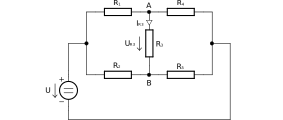
\includegraphics[width=0.8\columnwidth,keepaspectratio]{res/u2o1}
\end{center}
\subsection{Riešenie}
Vytvoríme si náhradný obvod: 
\begin{center}
  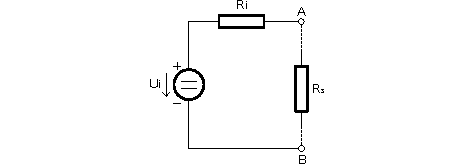
\includegraphics[width=0.8\columnwidth,keepaspectratio]{res/u2o2}
\end{center}
\begin{align*}
I_{R3} = \frac{U_{i}}{R_{3} + R_{i}}
\end{align*}
Výpočet odporu $R_{i}$ v náhradnom v obvode:
\begin{center}
  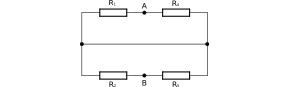
\includegraphics[width=0.8\columnwidth,keepaspectratio]{res/u2o3}
\end{center}
\begin{align*}
R_{i} = R_{AB} = \frac{R_{1} . R_{4}}{R_{1} + R_{4}} + \frac{R_{2} . R_{5}}{R_{2} + R_{5}}
\end{align*}
Výpočet napätia $U_{i}$ v náhradnom v obvode:
\begin{center}
  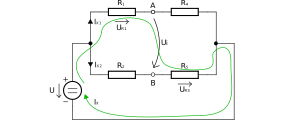
\includegraphics[width=0.8\columnwidth,keepaspectratio]{res/u2o4}
\end{center}
Vytvoríme si v obvode slučku aby sme mohli vypočítať napätie $U_{i}$ a zostavíme pre ňu rovnicu:
\begin{align*}
  U_{R1} + U_{i} + U_{R5} - U &= 0 \\
  I_{X1}.R_{1} + U_{i} + I_{X2}.R_{5} - U &= 0 \\
   U_{i} &=U -I_{X1}.R_{1}- I_{X2}.R_{5}
\end{align*}
Potrebujeme vypočítať $I_{X1}$ a $I_{X2}$, to urobíme pomocou metody slučkových prúdov:\\
\begin{minipage}{0.5\linewidth}
\begin{align*}
    U_{R1} + U_{R4} - U &= 0 \\
    R_{2}I_{X1} + R_{5}I_{X1} &= U \\
    I_{X1}(R_{2} + R_{5}) &= U \\
    I_{X1} &= \frac{U}{R_{2} + R_{5}} \\
\end{align*}
\end{minipage}
\begin{minipage}{0.45\linewidth}
\begin{align*}
    U_{R2} + U_{R5} - U &= 0 \\
    R_{1}I_{X2} + R_{4}I_{X2} &= U \\
    I_{X2}(R_{1} + R_{4}) &= U \\
    I_{X2} &= \frac{U}{R_{1} + R_{4}} \\
\end{align*}
\end{minipage}
\\
Dosadíme $I_{X1}$ a $I_{X2}$ do pôvodnej rovnice a vyjadríme si $U_{i}$: 
\begin{align*}
  U_{i} &= U - R_{1}.\frac{U}{R_{1} + R_{4}} - R_{5}.\frac{U}{R_{2} + R_{5}} \\
  U_{i} &= U . \left(1 - \frac{R_{1}}{R_{1} + R_{4}} - \frac{R_{5}}{R_{2} + R_{5}}\right)
\end{align*}
Máme všetky potrebné hodnoty pre výpočet $I_{R3}$. Dosadíme a vypočítame:
\begin{align*}
I_{R3} = \frac{U_{i}}{R_{3} + R_{i}} = \frac{U . \left(1 - \frac{R_{1}}{R_{1} + R_{4}} - \frac{R_{5}}{R_{2} + R_{5}}\right)}{R_{R3} + \frac{R_{1} . R_{4}}{R_{1} + R_{4}} + \frac{R_{2} . R_{5}}{R_{2} + R_{5}}} = \frac{50 . \left(1 - \frac{525}{525 + 530} - \frac{130}{620 + 130}\right)}{210 + \frac{525 . 530}{525 + 530} + \frac{620 . 130}{620 + 130}} = 0,0283~A
\end{align*}
Z prúdu $I_{R3}$ vypočítame aj napätie $U_{R3}$: 
\begin{align*}
U_{R3} = R_{3}.I_{R3} = 210.0,028306 = 5,9463~V
\end{align*}
\newpage
